% Capitolul 3: Modele ARIMA pentru Date Nestaționare
% Prezentare Beamer Cuprinzătoare
% Program de licență, Academia de Studii Economice din București

\documentclass[9pt, aspectratio=169, t]{beamer}

% Asigură încadrarea conținutului pe diapozitive
\setbeamersize{text margin left=8mm, text margin right=8mm}

%=============================================================================
% CONFIGURARE TEMĂ ȘI STIL
%=============================================================================
\usetheme{Madrid}
\usecolortheme{seahorse}

% Paletă de Culori Inspirată IDA
\definecolor{MainBlue}{RGB}{26, 58, 110}
\definecolor{AccentBlue}{RGB}{42, 82, 140}
\definecolor{IDAred}{RGB}{220, 53, 69}
\definecolor{DarkGray}{RGB}{51, 51, 51}
\definecolor{MediumGray}{RGB}{128, 128, 128}
\definecolor{LightGray}{RGB}{248, 248, 248}
\definecolor{VeryLightGray}{RGB}{235, 235, 235}
\definecolor{Crimson}{RGB}{220, 53, 69}
\definecolor{Forest}{RGB}{46, 125, 50}
\definecolor{Amber}{RGB}{181, 133, 63}

\setbeamercolor{palette primary}{bg=MainBlue, fg=white}
\setbeamercolor{palette secondary}{bg=MainBlue!85, fg=white}
\setbeamercolor{palette tertiary}{bg=MainBlue!70, fg=white}
\setbeamercolor{structure}{fg=MainBlue}
\setbeamercolor{title}{fg=MainBlue}
\setbeamercolor{frametitle}{fg=MainBlue, bg=white}
\setbeamercolor{block title}{bg=MainBlue, fg=white}
\setbeamercolor{block body}{bg=VeryLightGray, fg=DarkGray}
\setbeamercolor{block title alerted}{bg=Crimson, fg=white}
\setbeamercolor{block body alerted}{bg=Crimson!8, fg=DarkGray}
\setbeamercolor{block title example}{bg=Forest, fg=white}
\setbeamercolor{block body example}{bg=Forest!8, fg=DarkGray}
\setbeamercolor{item}{fg=MainBlue}

\setbeamertemplate{navigation symbols}{}

\setbeamertemplate{footline}{
    \leavevmode%
    \hbox{%
        \begin{beamercolorbox}[wd=.333333\paperwidth,ht=2.5ex,dp=1ex,center]{author in head/foot}%
            \usebeamerfont{author in head/foot}\insertshortauthor
        \end{beamercolorbox}%
        \begin{beamercolorbox}[wd=.333333\paperwidth,ht=2.5ex,dp=1ex,center]{title in head/foot}%
            \usebeamerfont{title in head/foot}\insertshorttitle
        \end{beamercolorbox}%
        \begin{beamercolorbox}[wd=.333333\paperwidth,ht=2.5ex,dp=1ex,right]{date in head/foot}%
            \usebeamerfont{date in head/foot}\insertshortdate{}\hspace*{2em}
            \insertframenumber{} / \inserttotalframenumber\hspace*{2ex}
        \end{beamercolorbox}}%
    \vskip0pt%
}

%=============================================================================
% PACHETE
%=============================================================================
\usepackage[utf8]{inputenc}
\usepackage[T1]{fontenc}
\usepackage{amsmath, amssymb, amsthm}
\usepackage{mathtools}
\usepackage{bm}
\usepackage{tikz}
\usetikzlibrary{arrows.meta, positioning, shapes, calc}
\usepackage{booktabs}
\usepackage{multirow}
\usepackage{array}
\usepackage{graphicx}
\usepackage{hyperref}
\hypersetup{colorlinks=false, pdfborder={0 0 0}}
\graphicspath{{../logos/}{../charts/}}

%=============================================================================
% MEDII PENTRU TEOREME
%=============================================================================
\theoremstyle{definition}
\setbeamertemplate{theorems}[numbered]
\newtheorem{defn}{Definiție}
\newtheorem{thm}{Teoremă}
\newtheorem{prop}{Propoziție}
\newtheorem{rmk}{Observație}

%=============================================================================
% COMENZI PERSONALIZATE
%=============================================================================
\newcommand{\E}{\mathbb{E}}
\newcommand{\Var}{\text{Var}}
\newcommand{\Cov}{\text{Cov}}
\newcommand{\Corr}{\text{Corr}}
\newcommand{\R}{\mathbb{R}}
\newcommand{\N}{\mathbb{N}}
\newcommand{\Z}{\mathbb{Z}}
\newcommand{\B}{\mathbf{B}}
\newcommand{\imark}{\textcolor{MainBlue}{\textbullet}}

%=============================================================================
% INFORMAȚII TITLU
%=============================================================================
\title[Capitolul 3: Modele ARIMA]{Capitolul 3: Modele ARIMA pentru Date Nestaționare}
\subtitle{Program de licență, Facultatea de Cibernetică, Statistică și Informatică Economică, Academia de Studii Economice din București}
\author[Prof. dr. Daniel Traian Pele]{Prof. dr. Daniel Traian Pele\\[0.2cm]\footnotesize\texttt{danpele@ase.ro}}
\institute{Academia de Studii Economice din București}
\date{An Universitar 2025--2026}

\begin{document}

%=============================================================================
% DIAPOZITIV TITLU
%=============================================================================
\begin{frame}[plain]
    \begin{tikzpicture}[remember picture, overlay]
        \fill[IDAred] (current page.north west) rectangle ([yshift=-0.15cm]current page.north east);
        \node[anchor=north west] at ([xshift=0.5cm, yshift=-0.3cm]current page.north west) {
            \href{https://www.ase.ro}{\includegraphics[height=1.1cm]{ase_logo.png}}
        };
        \node[anchor=north] at ([yshift=-0.3cm]current page.north) {
            \href{https://ai4efin.ase.ro}{\includegraphics[height=1.1cm]{ai4efin_logo.png}}
        };
        \node[anchor=north east] at ([xshift=-0.5cm, yshift=-0.3cm]current page.north east) {
            \href{https://www.digital-finance-msca.com}{\includegraphics[height=1.1cm]{msca_logo.png}}
        };
    \end{tikzpicture}
    \vfill
    \begin{center}
        {\Large\textcolor{MediumGray}{Analiza și Prognoza Seriilor de Timp}}\\[0.3cm]
        {\Huge\textbf{\textcolor{MainBlue}{Capitolul 3: Modele ARIMA}}}\\[0.5cm]
        {\Large\textcolor{IDAred}{Serii de Timp Nestaționare}}
    \end{center}
    \vfill

    \begin{tikzpicture}[remember picture, overlay]
        \fill[IDAred] (current page.south west) rectangle ([yshift=0.15cm]current page.south east);
        \node[anchor=south west] at ([xshift=0.5cm, yshift=0.8cm]current page.south west) {
            \href{https://theida.net}{\includegraphics[height=0.9cm]{ida_logo.png}}
        };
        \node[anchor=south] at ([xshift=-3cm, yshift=0.8cm]current page.south) {
            \href{https://blockchain-research-center.com}{\includegraphics[height=0.9cm]{brc_logo.png}}
        };
        \node[anchor=south] at ([yshift=0.8cm]current page.south) {
            \href{https://quantinar.com}{\includegraphics[height=0.9cm]{qr_logo.png}}
        };
        \node[anchor=south] at ([xshift=3cm, yshift=0.8cm]current page.south) {
            \href{https://quantlet.com}{\includegraphics[height=0.9cm]{ql_logo.png}}
        };
        \node[anchor=south east] at ([xshift=-0.5cm, yshift=0.8cm]current page.south east) {
            \href{https://ipe.ro/new}{\includegraphics[height=0.9cm]{acad_logo.png}}
        };
    \end{tikzpicture}
\end{frame}

%=============================================================================
% CUPRINS
%=============================================================================
\begin{frame}{Structura Cursului}
    \vspace{-0.3cm}
    {\small
    \begin{columns}[T]
        \begin{column}{0.48\textwidth}
            \tableofcontents[sections={1-6}, hideallsubsections]
        \end{column}
        \begin{column}{0.48\textwidth}
            \tableofcontents[sections={7-11}, hideallsubsections]
        \end{column}
    \end{columns}
    }
\end{frame}

%=============================================================================
% MOTIVAȚIE
%=============================================================================
\begin{frame}{Exemplu Motivațional: Datele Nestaționare Sunt Pretutindeni}
    \vspace{-0.3cm}
    \begin{center}
        \includegraphics[width=0.88\textwidth, height=0.62\textheight, keepaspectratio]{ch3_motivation_nonstationary.pdf}
    \end{center}
    \vspace{-0.2cm}
    {\footnotesize
    \begin{itemize}
        \item Prețurile acțiunilor, PIB, cursurile de schimb prezintă \textbf{trenduri} sau \textbf{comportament rătăcitor}
        \item Media din eșantion (linia roșie) este lipsită de sens pentru un mers aleatoriu
        \item Modelele ARMA standard \textbf{nu pot} gestiona aceste serii direct
    \end{itemize}
    }
\end{frame}

\begin{frame}{Aplicații Practice}
    \vspace{-0.3cm}
    \begin{center}
        \includegraphics[width=0.92\textwidth, height=0.58\textheight, keepaspectratio]{ch3_motivation_realworld.pdf}
    \end{center}
    \vspace{-0.2cm}
    {\footnotesize
    \begin{alertblock}{Provocarea}
        Datele financiare și economice sunt de obicei \textbf{integrate} (I(1) sau aproape de rădăcină unitate):
        \begin{itemize}
            \item Prețuri de acțiuni: mers aleatoriu în logaritmi
            \item Cursuri de schimb: mers aleatoriu
            \item Rate ale dobânzii: foarte persistente (aproape de rădăcină unitate)
        \end{itemize}
    \end{alertblock}
    }
\end{frame}

\begin{frame}{Soluția: Diferențierea}
    \vspace{-0.3cm}
    \begin{center}
        \includegraphics[width=0.88\textwidth, height=0.62\textheight, keepaspectratio]{ch3_motivation_differencing.pdf}
    \end{center}
    \vspace{-0.2cm}
    {\footnotesize
    \begin{exampleblock}{Observație Cheie}
        \textbf{Diferențierea} transformă o serie nestaționară într-una staționară:
        $\Delta Y_t = Y_t - Y_{t-1}$. ACF se schimbă de la descreștere lentă la descreștere rapidă!
    \end{exampleblock}
    }
\end{frame}

\begin{frame}{Ce Vom Învăța Astăzi}
    \begin{block}{Concepte Fundamentale}
        \begin{enumerate}
            \item \textbf{Nestaționaritatea}: De ce contează și cum o detectăm
            \item \textbf{Teste de Rădăcină Unitate}: Testele ADF, PP, KPSS
            \item \textbf{Diferențierea}: Transformarea cheie
            \item \textbf{Modele ARIMA}: Combinarea diferențierii cu ARMA
            \item \textbf{Metodologia Box-Jenkins}: Identificare $\to$ Estimare $\to$ Diagnosticare
        \end{enumerate}
    \end{block}

    \vspace{0.2cm}

    \begin{exampleblock}{La Sfârșitul Acestui Curs}
        Veți fi capabili să modelați și să prognozați serii de timp nestaționare precum prețurile acțiunilor, PIB și cursurile de schimb folosind modele ARIMA.
    \end{exampleblock}
\end{frame}

%=============================================================================
% SECȚIUNEA 1: NESTAȚIONARITATEA
%=============================================================================
\section{Nestaționaritatea în Seriile de Timp}

\begin{frame}{De Ce Contează Nestaționaritatea}
    {\small
    \hfill\begin{minipage}{0.9\textwidth}
    \begin{alertblock}{Problema}
        Multe serii de timp economice și financiare sunt \textbf{nestaționare}:
        \begin{itemize}\setlength{\itemsep}{0pt}
            \item PIB, prețuri de acțiuni, cursuri de schimb, indici de inflație
            \item Prezintă trenduri, medii în schimbare sau varianță în creștere
        \end{itemize}
    \end{alertblock}

    \vspace{0.1cm}

    \begin{block}{Consecințele Nestaționarității}
        \begin{itemize}\setlength{\itemsep}{0pt}
            \item Modelele ARMA standard presupun staționaritate
            \item Regresia OLS cu date nestaționare duce la \textbf{regresie falsă}
            \item Momentele din eșantion (medie, varianță, ACF) nu sunt estimatori consistenți
            \item Inferența statistică devine invalidă
        \end{itemize}
    \end{block}
    \end{minipage}
    }
\end{frame}

\begin{frame}{Exemplu: PIB Real SUA}
    \vspace{-0.3cm}
    \begin{center}
        \includegraphics[width=0.78\textwidth, height=0.55\textheight, keepaspectratio]{ch3_gdp_levels.pdf}
    \end{center}
    \vspace{-0.2cm}
    {\small
    \begin{itemize}
        \item \textbf{Trend} ascendent clar -- media nu este constantă
        \item Acesta este un exemplu clasic de serie de timp \textbf{nestaționară}
        \item Nu putem aplica modele ARMA direct pe aceste date
    \end{itemize}
    }
\end{frame}

\begin{frame}{Tipuri de Nestaționaritate}
    \begin{columns}[T]
        \begin{column}{0.48\textwidth}
            \begin{block}{Trend Determinist}
                $$Y_t = \alpha + \beta t + \varepsilon_t$$
                \begin{itemize}
                    \item Trendul este o funcție deterministă de timp
                    \item Poate fi eliminat prin \textbf{regresie}
                    \item Șocurile au efecte temporare
                \end{itemize}
            \end{block}
        \end{column}
        \begin{column}{0.48\textwidth}
            \begin{block}{Trend Stochastic (Rădăcină Unitate)}
                $$Y_t = Y_{t-1} + \varepsilon_t$$
                \begin{itemize}
                    \item Proces de mers aleatoriu
                    \item Trebuie eliminat prin \textbf{diferențiere}
                    \item Șocurile au efecte permanente
                \end{itemize}
            \end{block}
        \end{column}
    \end{columns}

    \vspace{0.5cm}

    \begin{alertblock}{Distincție Cheie}
        Identificarea corectă este crucială: eliminarea trendului prin regresie pentru un proces cu rădăcină unitate sau diferențierea unui proces staționar în trend duc ambele la specificare greșită!
    \end{alertblock}
\end{frame}

\begin{frame}{Vizualizarea Diferenței}
    \vspace{-0.3cm}
    \begin{center}
        \includegraphics[width=0.82\textwidth, height=0.58\textheight, keepaspectratio]{ch3_trend_comparison.pdf}
    \end{center}
    \vspace{-0.2cm}
    {\footnotesize
    \begin{itemize}
        \item \textbf{Stânga}: Trend determinist -- abaterile de la trend sunt temporare
        \item \textbf{Dreapta}: Trend stochastic -- șocurile se acumulează permanent
        \item Ambele arată similar, dar necesită tratamente \textbf{diferite}!
    \end{itemize}
    }
\end{frame}

\begin{frame}{Procesul de Mers Aleatoriu}
    {\small
    \hfill\begin{minipage}{0.9\textwidth}
    \begin{defn}[Mers Aleatoriu]
        Un \textbf{mers aleatoriu} este definit ca:
        $$Y_t = Y_{t-1} + \varepsilon_t, \quad \varepsilon_t \sim WN(0, \sigma^2)$$
        Cu condiția inițială $Y_0 = 0$, avem: $Y_t = \sum_{i=1}^{t} \varepsilon_i$
    \end{defn}

    \vspace{0.1cm}

    \begin{block}{Proprietățile Mersului Aleatoriu}
        \begin{itemize}\setlength{\itemsep}{0pt}
            \item $\E[Y_t] = 0$ (medie constantă)
            \item $\Var(Y_t) = t\sigma^2$ (varianța crește în timp!)
            \item $\Cov(Y_t, Y_{t-k}) = (t-k)\sigma^2$ pentru $k \leq t$
            \item ACF: $\rho_k = \sqrt{\frac{t-k}{t}} \to 1$ când $t \to \infty$
        \end{itemize}
    \end{block}
    \end{minipage}
    }
\end{frame}

\begin{frame}{Mers Aleatoriu: Ilustrație Vizuală}
    \begin{center}
        \includegraphics[width=0.95\textwidth]{ch3_def_random_walk.pdf}
    \end{center}
    \vspace{-0.2cm}
    \small Stânga: traiectorii multiple de mers aleatoriu rătăcesc imprevizibil. Dreapta: varianța crește liniar în timp.
\end{frame}

\begin{frame}{Mers Aleatoriu cu Drift}
    {\small
    \hfill\begin{minipage}{0.9\textwidth}
    \begin{defn}[Mers Aleatoriu cu Drift]
        Un mers aleatoriu cu drift include un termen constant:
        $$Y_t = \mu + Y_{t-1} + \varepsilon_t$$
        Echivalent: $Y_t = Y_0 + \mu t + \sum_{i=1}^{t} \varepsilon_i$
    \end{defn}

    \vspace{0.1cm}

    \begin{block}{Proprietăți}
        \begin{itemize}\setlength{\itemsep}{0pt}
            \item $\E[Y_t] = Y_0 + \mu t$ (media crește liniar)
            \item $\Var(Y_t) = t\sigma^2$ (varianța tot crește)
            \item Drift-ul $\mu$ creează un trend ascendent sau descendent
            \item Tot nestaționar în ciuda faptului că are un ``trend''
        \end{itemize}
    \end{block}
    \end{minipage}
    }
\end{frame}

\begin{frame}{Mers Aleatoriu cu Drift: Ilustrație Vizuală}
    \begin{center}
        \includegraphics[width=0.9\textwidth]{ch3_def_random_walk_drift.pdf}
    \end{center}
    \vspace{-0.2cm}
    \small Mersul aleatoriu fără drift (albastru) rătăcește în jurul lui zero. Cu drift (roșu), există un trend sistematic.
\end{frame}

\begin{frame}{Simularea Mersurilor Aleatorii}
    \vspace{-0.3cm}
    \begin{center}
        \includegraphics[width=0.82\textwidth, height=0.58\textheight, keepaspectratio]{ch3_random_walk.pdf}
    \end{center}
    \vspace{-0.2cm}
    {\footnotesize
    \begin{itemize}
        \item \textbf{Stânga}: Mersuri aleatorii pure -- fără drift, rătăcesc imprevizibil
        \item \textbf{Dreapta}: Mersuri aleatorii cu drift -- trend ascendent în medie
        \item Fiecare traiectorie este unică; incertitudinea crește în timp
    \end{itemize}
    }
\end{frame}

\begin{frame}{Creșterea Varianței: De Ce Mersurile Aleatorii Sunt Nestaționare}
    \vspace{-0.3cm}
    \begin{center}
        \includegraphics[width=0.82\textwidth, height=0.58\textheight, keepaspectratio]{ch3_variance_growth.pdf}
    \end{center}
    \vspace{-0.2cm}
    {\footnotesize
    \begin{itemize}
        \item \textbf{Stânga}: Evantaiul de traiectorii arată incertitudinea crescând în timp
        \item \textbf{Dreapta}: Varianța crește liniar: $\Var(Y_t) = t\sigma^2$
        \item Aceasta violează staționaritatea (varianța ar trebui să fie constantă)
    \end{itemize}
    }
\end{frame}

\begin{frame}{Procese Integrate}
    {\small
    \hfill\begin{minipage}{0.9\textwidth}
    \begin{defn}[Proces Integrat de Ordin $d$]
        O serie de timp $\{Y_t\}$ este \textbf{integrată de ordin $d$}, scrisă $Y_t \sim I(d)$, dacă:
        \begin{itemize}\setlength{\itemsep}{0pt}
            \item $Y_t$ este nestaționară
            \item $(1-L)^d Y_t = \Delta^d Y_t$ este staționară
            \item $(1-L)^{d-1} Y_t$ este încă nestaționară
        \end{itemize}
    \end{defn}

    \vspace{0.1cm}

    \begin{exampleblock}{Cazuri Comune}
        \begin{itemize}\setlength{\itemsep}{0pt}
            \item $I(0)$: Proces staționar (de ex., ARMA)
            \item $I(1)$: Prima diferență este staționară (cel mai frecvent pentru date economice)
            \item $I(2)$: A doua diferență este staționară (mai rar)
        \end{itemize}
    \end{exampleblock}
    \end{minipage}
    }
\end{frame}

\begin{frame}{Proces Integrat: Ilustrație Vizuală}
    \begin{center}
        \includegraphics[width=0.95\textwidth]{ch3_def_integrated.pdf}
    \end{center}
    \vspace{-0.2cm}
    \small $I(0)$: staționar. $I(1)$: o diferență necesară. $I(2)$: două diferențe necesare.
\end{frame}

%=============================================================================
% SECȚIUNEA 2: DIFERENȚIEREA
%=============================================================================
\section{Diferențierea și Operatorul Diferență}

\begin{frame}{Operatorul Diferență}
    {\small
    \hfill\begin{minipage}{0.9\textwidth}
    \begin{defn}[Prima Diferență]
        \textbf{Operatorul primei diferențe} $\Delta$ este definit ca:
        $\Delta Y_t = Y_t - Y_{t-1} = (1-L)Y_t$, unde $L$ este operatorul lag ($LY_t = Y_{t-1}$).
    \end{defn}

    \vspace{0.1cm}

    \begin{block}{Diferențe de Ordin Superior}
        \begin{itemize}\setlength{\itemsep}{0pt}
            \item A doua diferență: $\Delta^2 Y_t = \Delta(\Delta Y_t) = (1-L)^2 Y_t$
            \item $\Delta^2 Y_t = Y_t - 2Y_{t-1} + Y_{t-2}$
            \item Diferența de ordin $d$: $\Delta^d Y_t = (1-L)^d Y_t$
        \end{itemize}
    \end{block}

    \vspace{0.1cm}

    \begin{alertblock}{Rezultat Cheie}
        Dacă $Y_t \sim I(d)$, atunci $\Delta^d Y_t \sim I(0)$ (staționar).
    \end{alertblock}
    \end{minipage}
    }
\end{frame}

\begin{frame}{Prima Diferență: Ilustrație Vizuală}
    \begin{center}
        \includegraphics[width=0.95\textwidth]{ch3_def_difference.pdf}
    \end{center}
    \vspace{-0.2cm}
    \small Stânga: serie nestaționară. Dreapta: după prima diferență, seria devine staționară.
\end{frame}

\begin{frame}{Exemplu: Diferențierea unui Mers Aleatoriu}
    {\small
    \hfill\begin{minipage}{0.9\textwidth}
    \begin{exampleblock}{Mers Aleatoriu la Zgomot Alb}
        Fie $Y_t = Y_{t-1} + \varepsilon_t$ (mers aleatoriu). Luând prima diferență:
        $$\Delta Y_t = Y_t - Y_{t-1} = \varepsilon_t$$
        Prima diferență este zgomot alb -- un proces staționar!
    \end{exampleblock}

    \vspace{0.1cm}

    \begin{block}{Interpretare}
        \begin{itemize}\setlength{\itemsep}{0pt}
            \item Un mers aleatoriu este $I(1)$
            \item O diferență îl transformă în $I(0)$
            \item ``Schimbările'' într-un mers aleatoriu sunt staționare
        \end{itemize}
    \end{block}
    \end{minipage}
    }
\end{frame}

\begin{frame}{Diagnostic ACF: Detectarea Nestaționarității}
    \vspace{-0.3cm}
    \begin{center}
        \includegraphics[width=0.92\textwidth, height=0.68\textheight, keepaspectratio]{ch3_acf_nonstationary.pdf}
    \end{center}
    \vspace{-0.2cm}
    {\footnotesize
    \begin{itemize}
        \item \textbf{Sus}: ACF mers aleatoriu scade foarte lent $\Rightarrow$ rădăcină unitate
        \item \textbf{Jos}: După diferențiere, ACF se întrerupe $\Rightarrow$ staționar
    \end{itemize}
    }
\end{frame}

\begin{frame}{Diferențierea în Practică: Exemplul PIB}
    \vspace{-0.3cm}
    \begin{center}
        \includegraphics[width=0.92\textwidth, height=0.65\textheight, keepaspectratio]{ch3_differencing.pdf}
    \end{center}
    \vspace{-0.2cm}
    {\footnotesize
    \begin{itemize}
        \item \textbf{Stânga}: PIB în niveluri -- trend ascendent clar (nestaționar)
        \item \textbf{Dreapta}: Rata de creștere PIB (diferența logaritmică) -- fluctuează în jurul mediei (staționar)
        \item Diferențierea elimină trendul și obține staționaritate
    \end{itemize}
    }
\end{frame}

\begin{frame}{Supra-diferențierea}
    {\small
    \hfill\begin{minipage}{0.9\textwidth}
    \begin{alertblock}{Avertisment: Supra-diferențierea}
        Diferențierea mai mult decât este necesar introduce probleme:
        \begin{itemize}\setlength{\itemsep}{0pt}
            \item Creează autocorelație negativă artificială
            \item Inflează varianța
            \item Pierde informație
        \end{itemize}
    \end{alertblock}

    \vspace{0.1cm}

    \begin{exampleblock}{Exemplu}
        Dacă $Y_t \sim I(1)$, atunci $\Delta Y_t \sim I(0)$. Dar dacă diferențiem din nou:
        $$\Delta^2 Y_t = \Delta Y_t - \Delta Y_{t-1} = \varepsilon_t - \varepsilon_{t-1}$$
        Acesta este un MA(1) cu $\theta = 1$ (la granița non-invertibilității)!
    \end{exampleblock}
    \end{minipage}
    }
\end{frame}

%=============================================================================
% SECȚIUNEA 3: MODELE ARIMA
%=============================================================================
\section{Modele ARIMA(p,d,q)}

\begin{frame}{Definiția ARIMA}
    {\small
    \hfill\begin{minipage}{0.9\textwidth}
    \begin{defn}[ARIMA(p,d,q)]
        O serie de timp $\{Y_t\}$ urmează un proces \textbf{ARIMA(p,d,q)} dacă:
        $$\phi(L)(1-L)^d Y_t = c + \theta(L)\varepsilon_t$$
        unde:
        \begin{itemize}\setlength{\itemsep}{0pt}
            \item $\phi(L) = 1 - \phi_1 L - \phi_2 L^2 - \cdots - \phi_p L^p$ (polinomul AR)
            \item $\theta(L) = 1 + \theta_1 L + \theta_2 L^2 + \cdots + \theta_q L^q$ (polinomul MA)
            \item $d$ este ordinul de integrare (numărul de diferențe)
            \item $\varepsilon_t \sim WN(0, \sigma^2)$
        \end{itemize}
    \end{defn}
    \end{minipage}
    }
\end{frame}

\begin{frame}{ARIMA: Ilustrație Vizuală}
    \begin{center}
        \includegraphics[width=0.85\textwidth, height=0.62\textheight, keepaspectratio]{ch3_def_arima.pdf}
    \end{center}
    \vspace{-0.2cm}
    \small Sus: seria ARIMA originală. Jos stânga/dreapta: după diferențiere, ACF/PACF ajută la identificarea ordinelor AR și MA.
\end{frame}

\begin{frame}{Componentele ARIMA}
    \begin{center}
        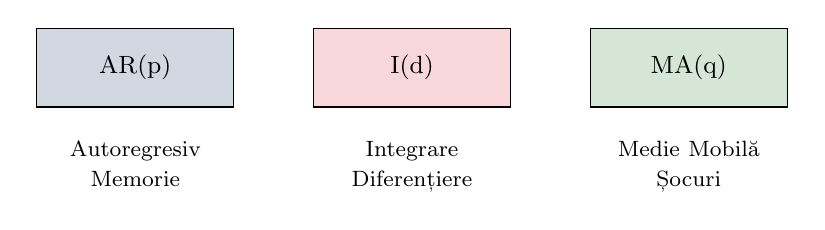
\begin{tikzpicture}[node distance=2cm, every node/.style={font=\small}]
            \node[draw, rectangle, fill=MainBlue!20, minimum width=2.5cm, minimum height=1cm] (AR) {AR(p)};
            \node[draw, rectangle, fill=Crimson!20, minimum width=2.5cm, minimum height=1cm, right=1cm of AR] (I) {I(d)};
            \node[draw, rectangle, fill=Forest!20, minimum width=2.5cm, minimum height=1cm, right=1cm of I] (MA) {MA(q)};

            \node[below=0.3cm of AR, text width=2.5cm, align=center] {\footnotesize Autoregresiv\\Memorie};
            \node[below=0.3cm of I, text width=2.5cm, align=center] {\footnotesize Integrare\\Diferențiere};
            \node[below=0.3cm of MA, text width=2.5cm, align=center] {\footnotesize Medie Mobilă\\Șocuri};
        \end{tikzpicture}
    \end{center}

    \vspace{0.2cm}

    {\small
    \begin{block}{Cazuri Speciale}
        \begin{itemize}\setlength{\itemsep}{0pt}
            \item ARIMA(p,0,q) = ARMA(p,q) -- staționar
            \item ARIMA(0,1,0) = Mers aleatoriu
            \item ARIMA(0,1,1) = IMA(1,1) -- netezire exponențială
            \item ARIMA(1,1,0) = ARI(1,1) -- AR(1) diferențiat
        \end{itemize}
    \end{block}
    }
\end{frame}

\begin{frame}{Exemplu ARIMA(1,1,0)}
    {\small
    \hfill\begin{minipage}{0.9\textwidth}
    \begin{exampleblock}{Model ARI(1,1)}
        $$\Delta Y_t = c + \phi_1 \Delta Y_{t-1} + \varepsilon_t$$
        Echivalent: $(1-\phi_1 L)(1-L)Y_t = c + \varepsilon_t$
    \end{exampleblock}

    \vspace{0.1cm}

    \begin{block}{Interpretare}
        \begin{itemize}\setlength{\itemsep}{0pt}
            \item \textbf{Schimbările} în $Y_t$ urmează un proces AR(1)
            \item Dacă $|\phi_1| < 1$, schimbările sunt staționare
            \item $Y_t$ în sine are un trend stochastic
            \item Model comun pentru multe serii de timp economice
        \end{itemize}
    \end{block}
    \end{minipage}
    }
\end{frame}

\begin{frame}{Exemplu ARIMA(0,1,1)}
    {\small
    \hfill\begin{minipage}{0.9\textwidth}
    \begin{exampleblock}{Model IMA(1,1)}
        $$\Delta Y_t = c + \varepsilon_t + \theta_1 \varepsilon_{t-1}$$
        Echivalent: $(1-L)Y_t = c + (1+\theta_1 L)\varepsilon_t$
    \end{exampleblock}

    \vspace{0.1cm}

    \begin{block}{Conexiunea cu Netezirea Exponențială}
        Modelul IMA(1,1) este echivalent cu \textbf{netezirea exponențială simplă}:
        $$\hat{Y}_{t+1} = \alpha Y_t + (1-\alpha)\hat{Y}_t$$
        unde $\alpha = 1 + \theta_1$ (pentru $-1 < \theta_1 < 0$).
    \end{block}
    \end{minipage}
    }
\end{frame}

\begin{frame}{Rolul Constantei în ARIMA}
    {\small
    \hfill\begin{minipage}{0.9\textwidth}
    \begin{block}{Termenul Constant în ARIMA(p,d,q)}
        Când $d > 0$, constanta $c$ are o interpretare diferită:
        $\phi(L)(1-L)^d Y_t = c + \theta(L)\varepsilon_t$
    \end{block}

    \vspace{0.1cm}

    \begin{alertblock}{Implicații Importante}
        \begin{itemize}\setlength{\itemsep}{0pt}
            \item Pentru $d=1$: $c$ reprezintă \textbf{drift-ul} (schimbarea medie): $\E[\Delta Y_t] = \frac{c}{1-\phi_1-\cdots-\phi_p}$
            \item Pentru $d=2$: $c$ afectează \textbf{curbura} trendului
            \item Adesea se presupune $c=0$ când $d \geq 1$
        \end{itemize}
    \end{alertblock}
    \end{minipage}
    }
\end{frame}

%=============================================================================
% SECȚIUNEA 4: TESTE DE RĂDĂCINĂ UNITATE
%=============================================================================
\section{Teste de Rădăcină Unitate}

\begin{frame}{Testarea pentru Rădăcini Unitate}
    {\small
    \hfill\begin{minipage}{0.9\textwidth}
    \begin{block}{De Ce Testăm?}
        Înainte de a potrivi un model ARIMA, trebuie să determinăm:
        \begin{enumerate}\setlength{\itemsep}{0pt}
            \item Este seria staționară? (Este $d=0$?)
            \item Dacă nu, câte diferențe sunt necesare? (Care este $d$?)
        \end{enumerate}
    \end{block}

    \vspace{0.1cm}

    \begin{block}{Teste Comune de Rădăcină Unitate}
        \begin{itemize}\setlength{\itemsep}{0pt}
            \item \textbf{Dickey-Fuller (DF)} și \textbf{Augmented Dickey-Fuller (ADF)}
            \item \textbf{Phillips-Perron (PP)}
            \item \textbf{KPSS} (test de staționaritate -- ipoteză nulă inversată)
        \end{itemize}
    \end{block}
    \end{minipage}
    }
\end{frame}

\begin{frame}{Testul Dickey-Fuller}
    {\small
    \hfill\begin{minipage}{0.9\textwidth}
    \begin{block}{Configurare}
        Considerăm modelul AR(1): $Y_t = \phi Y_{t-1} + \varepsilon_t$. Scădem $Y_{t-1}$:
        $\Delta Y_t = (\phi - 1)Y_{t-1} + \varepsilon_t = \gamma Y_{t-1} + \varepsilon_t$, unde $\gamma = \phi - 1$.
    \end{block}

    \vspace{0.1cm}

    \begin{block}{Ipoteze}
        \begin{itemize}\setlength{\itemsep}{0pt}
            \item $H_0$: $\gamma = 0$ (rădăcină unitate, $\phi = 1$, nestaționar)
            \item $H_1$: $\gamma < 0$ (staționar, $|\phi| < 1$)
        \end{itemize}
    \end{block}

    \vspace{0.1cm}

    \begin{alertblock}{Problemă Cheie}
        Sub $H_0$, statistica $t$ \textbf{nu} urmează o distribuție $t$ standard! Trebuie folosite valorile critice Dickey-Fuller.
    \end{alertblock}
    \end{minipage}
    }
\end{frame}

\begin{frame}{Variante ale Testului Dickey-Fuller}
    {\small
    \hfill\begin{minipage}{0.9\textwidth}
    \begin{block}{Trei Specificări}
        \begin{enumerate}\setlength{\itemsep}{0pt}
            \item \textbf{Fără constantă, fără trend}: $\Delta Y_t = \gamma Y_{t-1} + \varepsilon_t$
            \item \textbf{Cu constantă (drift)}: $\Delta Y_t = \alpha + \gamma Y_{t-1} + \varepsilon_t$
            \item \textbf{Cu constantă și trend}: $\Delta Y_t = \alpha + \beta t + \gamma Y_{t-1} + \varepsilon_t$
        \end{enumerate}
    \end{block}

    \vspace{0.1cm}

    \begin{alertblock}{Alegerea Specificării Corecte}
        \begin{itemize}\setlength{\itemsep}{0pt}
            \item Examinați datele: au un trend vizibil?
            \item Includerea termenilor inutili reduce puterea
            \item Excluderea termenilor necesari duce la inferență incorectă
        \end{itemize}
    \end{alertblock}
    \end{minipage}
    }
\end{frame}

\begin{frame}{Testul Augmented Dickey-Fuller (ADF)}
    \vspace{-0.2cm}
    {\small
    \begin{block}{Problema cu DF Simplu}
        Dacă există dinamică AR dincolo de AR(1), reziduurile DF vor fi autocorelate.
    \end{block}

    \vspace{0.1cm}

    \begin{defn}[Testul ADF]
        Adăugați diferențe întârziate: $\Delta Y_t = \alpha + \beta t + \gamma Y_{t-1} + \sum_{j=1}^{k} \delta_j \Delta Y_{t-j} + \varepsilon_t$

        Testați $H_0: \gamma = 0$ folosind valorile critice ADF.
    \end{defn}

    \vspace{0.1cm}

    \begin{block}{Alegerea Lungimii Lag-ului $k$}
        \begin{itemize}
            \item Folosiți criterii informaționale (AIC, BIC)
            \item Începeți cu $k_{max}$, reduceți până ultimul lag este semnificativ
        \end{itemize}
    \end{block}
    }
\end{frame}

\begin{frame}{Testul ADF: Ilustrație Vizuală}
    \begin{center}
        \includegraphics[width=0.95\textwidth]{ch3_def_adf.pdf}
    \end{center}
    \vspace{-0.2cm}
    \small Stânga: serie staționară -- ADF respinge rădăcina unitate. Dreapta: nestaționară -- ADF nu respinge.
\end{frame}

\begin{frame}{Valori Critice ADF}
    \vspace{-0.2cm}
    {\small
    \begin{table}
        \centering
        \begin{tabular}{lccc}
            \toprule
            \textbf{Model} & \textbf{1\%} & \textbf{5\%} & \textbf{10\%} \\
            \midrule
            Fără constantă, fără trend & $-2.58$ & $-1.95$ & $-1.62$ \\
            Cu constantă & $-3.43$ & $-2.86$ & $-2.57$ \\
            Cu constantă și trend & $-3.96$ & $-3.41$ & $-3.13$ \\
            \bottomrule
        \end{tabular}
    \end{table}
    }
    \vspace{-0.1cm}
    \begin{block}{Regula de Decizie}
        {\small
        \begin{itemize}
            \item Statistică de test $<$ valoare critică $\Rightarrow$ Respingem $H_0$ (staționar)
            \item Statistică de test $\geq$ valoare critică $\Rightarrow$ Nu respingem (rădăcină unitate)
        \end{itemize}
        }
    \end{block}
\end{frame}

\begin{frame}{Testul Phillips-Perron (PP)}
    {\small
    \hfill\begin{minipage}{0.9\textwidth}
    \begin{block}{Motivație}
        Ca și ADF, testează $H_0$: Rădăcină unitate vs $H_1$: Staționar, dar folosește o \textbf{corecție non-parametrică} pentru corelația serială în loc de adăugarea diferențelor întârziate.
    \end{block}

    \begin{block}{Statistica de Test}
        Testul PP modifică statistica $t$ DF:
        $$Z_t = t_{\hat{\gamma}} \cdot \sqrt{\frac{\hat{\sigma}^2}{\hat{\lambda}^2}} - \frac{T(\hat{\lambda}^2 - \hat{\sigma}^2)(se(\hat{\gamma}))}{2\hat{\lambda}^2 \cdot s}$$
        unde $\hat{\lambda}^2$ este o estimare consistentă a varianței pe termen lung folosind Newey-West.
    \end{block}

    \begin{exampleblock}{Avantaje față de ADF}
        \begin{itemize}\setlength{\itemsep}{0pt}
            \item Robust la heteroscedasticitate și corelație serială
            \item Nu necesită selectarea lungimii lag-ului (folosește lățime de bandă)
        \end{itemize}
    \end{exampleblock}
    \end{minipage}
    }
\end{frame}

\begin{frame}{Testul KPSS}
    \vspace{-0.2cm}
    {\small
    \hfill\begin{minipage}{0.9\textwidth}
    \begin{block}{Ipoteze Inversate}
        Spre deosebire de ADF: $H_0$: Staționar \quad vs \quad $H_1$: Rădăcină unitate
    \end{block}

    \vspace{0.1cm}

    \begin{block}{Procedura KPSS}
        Descompunem: $Y_t = \xi t + r_t + \varepsilon_t$ unde $r_t = r_{t-1} + u_t$.
        Testăm dacă $\Var(u_t) = 0$.
    \end{block}

    \vspace{0.1cm}

    \begin{exampleblock}{Utilizare Complementară cu ADF}
        \begin{itemize}
            \item ADF respinge, KPSS nu respinge $\Rightarrow$ Staționar
            \item ADF nu respinge, KPSS respinge $\Rightarrow$ Rădăcină unitate
            \item Ambele resping sau niciunul $\Rightarrow$ Neconcludent
        \end{itemize}
    \end{exampleblock}
    \end{minipage}
    }
\end{frame}

%=============================================================================
% SECȚIUNEA 5: IDENTIFICAREA MODELULUI
%=============================================================================
\section{Identificarea Modelului ARIMA}

\begin{frame}{Metodologia Box-Jenkins}
    \begin{center}
        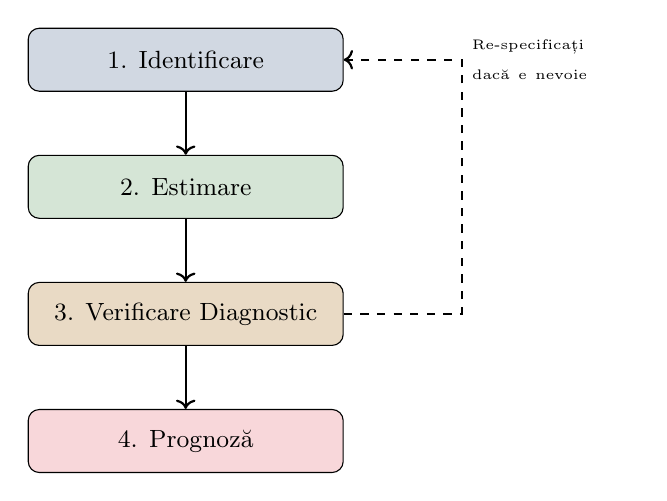
\begin{tikzpicture}[node distance=1.5cm, every node/.style={font=\small}]
            \node[draw, rectangle, rounded corners, fill=MainBlue!20, minimum width=4cm, minimum height=0.8cm] (id) {1. Identificare};
            \node[draw, rectangle, rounded corners, fill=Forest!20, minimum width=4cm, minimum height=0.8cm, below=0.8cm of id] (est) {2. Estimare};
            \node[draw, rectangle, rounded corners, fill=Amber!30, minimum width=4cm, minimum height=0.8cm, below=0.8cm of est] (diag) {3. Verificare Diagnostic};
            \node[draw, rectangle, rounded corners, fill=Crimson!20, minimum width=4cm, minimum height=0.8cm, below=0.8cm of diag] (fore) {4. Prognoză};

            \draw[->, thick] (id) -- (est);
            \draw[->, thick] (est) -- (diag);
            \draw[->, thick] (diag) -- (fore);
            \draw[->, thick, dashed] (diag.east) -- ++(1.5,0) |- (id.east) node[midway, right, text width=2cm] {\tiny Re-specificați dacă e nevoie};
        \end{tikzpicture}
    \end{center}
\end{frame}

\begin{frame}{Pasul 1: Determinarea lui $d$}
    {\small
    \hfill\begin{minipage}{0.9\textwidth}
    \begin{block}{Procedură}
        \begin{enumerate}\setlength{\itemsep}{0pt}
            \item Reprezentați grafic seria de timp -- căutați trenduri, varianță în schimbare
            \item Examinați ACF -- descreștere lentă sugerează nestaționaritate
            \item Aplicați teste de rădăcină unitate (ADF, KPSS)
            \item Dacă nestaționară, diferențiați și repetați
        \end{enumerate}
    \end{block}

    \vspace{0.1cm}

    \begin{exampleblock}{Ghiduri Practice}
        \begin{itemize}\setlength{\itemsep}{0pt}
            \item Majoritatea seriilor economice: $d = 1$ este suficient
            \item Rar avem nevoie de $d > 2$
            \item Dacă ACF al $\Delta Y_t$ tot scade lent, încercați $d = 2$
            \item Atenție la supra-diferențiere (ACF cu $\rho_1 \approx -0.5$)
        \end{itemize}
    \end{exampleblock}
    \end{minipage}
    }
\end{frame}

\begin{frame}{Pasul 2: Determinarea lui $p$ și $q$}
    \vspace{-0.2cm}
    {\small
    \hfill\begin{minipage}{0.92\textwidth}
    \begin{block}{După Diferențiere}
        Odată ce $W_t = \Delta^d Y_t$ este staționar, folosiți ACF/PACF pentru a identifica ARMA($p$,$q$):
    \end{block}

    \vspace{0.1cm}

    \begin{center}
        \begin{tabular}{lcc}
            \toprule
            \textbf{Model} & \textbf{ACF} & \textbf{PACF} \\
            \midrule
            AR($p$) & Scade exponențial & Se întrerupe după lag $p$ \\
            MA($q$) & Se întrerupe după lag $q$ & Scade exponențial \\
            ARMA($p$,$q$) & Scade & Scade \\
            \bottomrule
        \end{tabular}
    \end{center}

    \vspace{0.1cm}

    \begin{block}{Criterii Informaționale}
        Când tiparele sunt neclare, comparați modelele folosind:
        \begin{itemize}\setlength{\itemsep}{0pt}
            \item AIC = $-2\ln(L) + 2k$; \quad BIC = $-2\ln(L) + k\ln(n)$
        \end{itemize}
        Mai mic este mai bun. BIC penalizează complexitatea mai mult.
    \end{block}
    \end{minipage}
    }
\end{frame}

\begin{frame}{Algoritmi Auto-ARIMA}
    {\small
    \hfill\begin{minipage}{0.9\textwidth}
    \begin{block}{Selecție Automată a Modelului}
        Software-ul modern poate selecta automat $(p,d,q)$:
        \begin{itemize}\setlength{\itemsep}{0pt}
            \item Python: \texttt{pmdarima.auto\_arima()}
            \item R: \texttt{forecast::auto.arima()}
        \end{itemize}
    \end{block}

    \vspace{0.1cm}

    \begin{block}{Cum Funcționează Auto-ARIMA}
        \begin{enumerate}\setlength{\itemsep}{0pt}
            \item Folosește teste de rădăcină unitate pentru a determina $d$
            \item Potrivește modele pentru diverse combinații $(p,q)$
            \item Selectează modelul cu cel mai mic AIC/BIC
            \item Opțional folosește căutare pas cu pas pentru eficiență
        \end{enumerate}
    \end{block}

    \vspace{0.1cm}

    \begin{alertblock}{Atenție}
        Selecția automată este utilă dar nu infailibilă. Verificați întotdeauna diagnosticele!
    \end{alertblock}
    \end{minipage}
    }
\end{frame}

%=============================================================================
% SECȚIUNEA 6: ESTIMARE
%=============================================================================
\section{Estimarea ARIMA}

\begin{frame}{Metode de Estimare}
    {\small
    \hfill\begin{minipage}{0.9\textwidth}
    \begin{block}{Estimarea prin Maximum de Verosimilitate (MLE)}
        Abordarea standard pentru ARIMA:
        \begin{itemize}\setlength{\itemsep}{0pt}
            \item Presupune $\varepsilon_t \sim N(0, \sigma^2)$
            \item Maximizează funcția de verosimilitate
            \item Oferă estimatori consistenți, eficienți
            \item Furnizează erori standard pentru inferență
        \end{itemize}
    \end{block}

    \vspace{0.1cm}

    \begin{block}{MLE Condiționată vs Exactă}
        \begin{itemize}\setlength{\itemsep}{0pt}
            \item \textbf{MLE Condiționată}: Condiționează pe valorile inițiale
            \item \textbf{MLE Exactă}: Tratează valorile inițiale ca necunoscute
            \item Diferența diminuează pe măsură ce dimensiunea eșantionului crește
        \end{itemize}
    \end{block}
    \end{minipage}
    }
\end{frame}

\begin{frame}{Restricții asupra Parametrilor}
    {\small
    \hfill\begin{minipage}{0.9\textwidth}
    \begin{alertblock}{Staționaritate și Invertibilitate}
        Modelul ARIMA estimat ar trebui să satisfacă:
        \begin{itemize}\setlength{\itemsep}{0pt}
            \item \textbf{Staționaritate AR}: Rădăcinile lui $\phi(z) = 0$ în afara cercului unitate
            \item \textbf{Invertibilitate MA}: Rădăcinile lui $\theta(z) = 0$ în afara cercului unitate
        \end{itemize}
    \end{alertblock}

    \vspace{0.1cm}

    \begin{block}{Verificare în Practică}
        Majoritatea software-ului raportează:
        \begin{itemize}\setlength{\itemsep}{0pt}
            \item Coeficienți estimați cu erori standard
            \item Rădăcinile polinoamelor AR și MA
            \item Avertisment dacă este detectată aproape-rădăcină-unitate
        \end{itemize}
    \end{block}
    \end{minipage}
    }
\end{frame}

%=============================================================================
% SECȚIUNEA 7: DIAGNOSTICARE
%=============================================================================
\section{Verificare Diagnostic}

\begin{frame}{Analiza Reziduurilor}
    {\small
    \hfill\begin{minipage}{0.9\textwidth}
    \begin{block}{Ce Trebuie Verificat}
        Dacă modelul este corect, reziduurile $\hat{\varepsilon}_t$ ar trebui să fie zgomot alb:
        \begin{enumerate}\setlength{\itemsep}{0pt}
            \item Medie zero
            \item Varianță constantă
            \item Fără autocorelație
            \item (Opțional) Normalitate
        \end{enumerate}
    \end{block}

    \vspace{0.1cm}

    \begin{block}{Instrumente de Diagnostic}
        \begin{itemize}\setlength{\itemsep}{0pt}
            \item \textbf{ACF/PACF rezidual}: Nu ar trebui să arate vârfuri semnificative
            \item \textbf{Testul Ljung-Box}: Testează autocorelația la lag-uri multiple
            \item \textbf{Graficul Q-Q}: Verifică ipoteza de normalitate
            \item \textbf{Rezidual vs potrivit}: Verifică heteroscedasticitatea
        \end{itemize}
    \end{block}
    \end{minipage}
    }
\end{frame}

\begin{frame}{Testul Ljung-Box}
    {\small
    \hfill\begin{minipage}{0.9\textwidth}
    \begin{defn}[Statistica Q Ljung-Box]
        $Q(m) = n(n+2) \sum_{k=1}^{m} \frac{\hat{\rho}_k^2}{n-k}$. Sub $H_0$ (fără autocorelație): $Q(m) \sim \chi^2(m-p-q)$
    \end{defn}

    \vspace{0.1cm}

    \begin{block}{Utilizare}
        \begin{itemize}\setlength{\itemsep}{0pt}
            \item Alegeți $m \approx \ln(n)$ sau $m = 10$ pentru trimestrial, $m = 20$ pentru lunar
            \item Grade de libertate ajustate pentru parametrii estimați
            \item Respingeți dacă $Q(m)$ depășește valoarea critică
        \end{itemize}
    \end{block}

    \vspace{0.1cm}

    \begin{alertblock}{Dacă Testul Eșuează}
        Luați în considerare adăugarea de termeni AR sau MA, sau verificați pentru rupturi structurale.
    \end{alertblock}
    \end{minipage}
    }
\end{frame}

%=============================================================================
% SECȚIUNEA 8: PROGNOZA
%=============================================================================
\section{Prognoza cu ARIMA}

\begin{frame}{Prognoze Punctuale}
    {\small
    \hfill\begin{minipage}{0.9\textwidth}
    \begin{block}{Prognoza cu MSE Minim}
        Prognoza optimă la $h$ pași înainte este speranța condiționată:
        $\hat{Y}_{T+h|T} = \E[Y_{T+h} | Y_T, Y_{T-1}, \ldots]$
    \end{block}

    \vspace{0.1cm}

    \begin{exampleblock}{Prognoza ARIMA(1,1,1)}
        Model: $(1-\phi_1 L)(1-L)Y_t = c + (1+\theta_1 L)\varepsilon_t$

        Prognoză un pas: $\hat{Y}_{T+1|T} = c + Y_T + \phi_1(Y_T - Y_{T-1}) + \theta_1 \hat{\varepsilon}_T$

        Pentru $h > 1$: înlocuiți $\varepsilon_{T+j}$ necunoscut cu 0, $Y_{T+j}$ necunoscut cu $\hat{Y}_{T+j|T}$
    \end{exampleblock}
    \end{minipage}
    }
\end{frame}

\begin{frame}{Intervale de Prognoză}
    {\small
    \hfill\begin{minipage}{0.9\textwidth}
    \begin{block}{Incertitudinea Prognozei}
        Varianța erorii de prognoză la $h$ pași: $\Var(e_{T+h}) = \sigma^2 \sum_{j=0}^{h-1} \psi_j^2$, unde $\psi_j$ sunt coeficienții MA($\infty$).
    \end{block}

    \vspace{0.1cm}

    \begin{block}{Intervale de Încredere}
        Sub normalitate, interval $(1-\alpha)$\%: $\hat{Y}_{T+h|T} \pm z_{\alpha/2} \sqrt{\Var(e_{T+h})}$
    \end{block}

    \vspace{0.1cm}

    \begin{alertblock}{Proprietate Cheie pentru Serii I(1)}
        Pentru procese integrate, varianța prognozei crește nelimitat când $h \to \infty$. Intervalele se lărgesc în timp!
    \end{alertblock}
    \end{minipage}
    }
\end{frame}

\begin{frame}{Prognoze pe Termen Lung pentru ARIMA}
    {\small
    \hfill\begin{minipage}{0.9\textwidth}
    \begin{block}{Comportament când $h \to \infty$}
        Pentru ARIMA(p,1,q) cu drift $c$:
        \begin{itemize}\setlength{\itemsep}{0pt}
            \item Prognoze punctuale: Trend liniar cu pantă = drift
            \item Intervale de prognoză: Lățimea crește cu $\sqrt{h}$
        \end{itemize}

        Pentru ARIMA(p,1,q) fără drift:
        \begin{itemize}\setlength{\itemsep}{0pt}
            \item Prognoze punctuale: Converg la ultimul nivel
            \item Intervale de prognoză: Tot cresc nelimitat
        \end{itemize}
    \end{block}

    \vspace{0.1cm}

    \begin{alertblock}{Implicație Practică}
        Prognozele ARIMA sunt cele mai fiabile pentru orizonturi scurte. Prognozele pe termen lung au benzi de incertitudine foarte largi.
    \end{alertblock}
    \end{minipage}
    }
\end{frame}

\begin{frame}{Prognoză Rulantă: Concept}
    {\small
    \hfill\begin{minipage}{0.9\textwidth}
    \begin{block}{Ce este Prognoza Rulantă?}
        O tehnică pentru evaluarea acurateții prognozei în afara eșantionului:
        \begin{enumerate}\setlength{\itemsep}{0pt}
            \item Fixăm o \textbf{fereastră de antrenament} de dimensiune $w$
            \item Estimăm modelul pe observațiile $t = 1, \ldots, w$
            \item Prognozăm $h$ pași înainte: $\hat{Y}_{w+h|w}$
            \item \textbf{Deplasăm} fereastra înainte cu o perioadă
            \item Repetăm până la sfârșitul eșantionului
        \end{enumerate}
    \end{block}

    \vspace{0.1cm}

    \begin{exampleblock}{De ce Prognoze Rulante?}
        \begin{itemize}\setlength{\itemsep}{0pt}
            \item Mimează scenariul de prognoză în timp real
            \item Oferă multiple erori de prognoză pentru evaluare
            \item Evită supraajustarea pe întregul eșantion
        \end{itemize}
    \end{exampleblock}
    \end{minipage}
    }
\end{frame}

\begin{frame}{Prognoză Rulantă: Exemplu Pas cu Pas}
    \vspace{-0.2cm}
    {\footnotesize
    \begin{exampleblock}{Configurare: ARIMA(1,1,0) cu $\phi_1 = 0.6$}
        \vspace{-0.1cm}
        Model: $\Delta Y_t = \phi_1 \Delta Y_{t-1} + \varepsilon_t$ unde $\Delta Y_t = Y_t - Y_{t-1}$
        \vspace{-0.1cm}
    \end{exampleblock}

    \vspace{0.1cm}

    \begin{block}{Date la Momentul $T$}
        \vspace{-0.1cm}
        $Y_{T-2} = 100$, \quad $Y_{T-1} = 103$, \quad $Y_T = 108$ \quad $\Rightarrow$ \quad $\Delta Y_{T-1} = 3$, \quad $\Delta Y_T = 5$
        \vspace{-0.1cm}
    \end{block}

    \vspace{0.1cm}

    \begin{alertblock}{Prognoză Punctuală la 1 Pas}
        \vspace{-0.3cm}
        \begin{align*}
            \hat{\Delta Y}_{T+1|T} &= \phi_1 \cdot \Delta Y_T = 0.6 \times 5 = 3 \\[-0.2cm]
            \hat{Y}_{T+1|T} &= Y_T + \hat{\Delta Y}_{T+1|T} = 108 + 3 = \boxed{111}
        \end{align*}
        \vspace{-0.3cm}
    \end{alertblock}
    }
\end{frame}

\begin{frame}{Prognoze Punctuale Multi-Pas}
    \vspace{-0.2cm}
    {\footnotesize
    \begin{block}{Prognoză la 2 Pași}
        \vspace{-0.3cm}
        \begin{align*}
            \hat{\Delta Y}_{T+2|T} &= \phi_1 \cdot \hat{\Delta Y}_{T+1|T} = 0.6 \times 3 = 1.8 \\[-0.2cm]
            \hat{Y}_{T+2|T} &= \hat{Y}_{T+1|T} + \hat{\Delta Y}_{T+2|T} = 111 + 1.8 = \boxed{112.8}
        \end{align*}
        \vspace{-0.3cm}
    \end{block}

    \vspace{0.05cm}

    \begin{block}{Formula Generală pentru Prognoză la $h$ Pași (ARIMA(1,1,0))}
        \vspace{-0.3cm}
        \begin{align*}
            \hat{\Delta Y}_{T+h|T} &= \phi_1^h \cdot \Delta Y_T \\[-0.2cm]
            \hat{Y}_{T+h|T} &= Y_T + \Delta Y_T \cdot \frac{\phi_1(1-\phi_1^h)}{1-\phi_1}
        \end{align*}
        \vspace{-0.3cm}
    \end{block}

    \vspace{0.05cm}

    \begin{exampleblock}{Numeric: Prognoză la 3 Pași}
        \vspace{-0.1cm}
        $\hat{Y}_{T+3|T} = 108 + 5 \times \frac{0.6(1-0.6^3)}{1-0.6} = 108 + 5 \times 1.092 = \boxed{113.46}$
        \vspace{-0.1cm}
    \end{exampleblock}
    }
\end{frame}

\begin{frame}{Intervale de Încredere: Formule}
    {\small
    \hfill\begin{minipage}{0.9\textwidth}
    \begin{block}{Varianța Erorii de Prognoză}
        Pentru ARIMA(1,1,0), varianța erorii de prognoză la $h$ pași:
        $$\Var(e_{T+h|T}) = \sigma^2 \left(1 + \sum_{j=1}^{h-1} \psi_j^2 \right)$$
        unde $\psi_j = \phi_1^{j-1}(1 + \phi_1 + \cdots + \phi_1^{j-1}) = \phi_1^{j-1} \cdot \frac{1-\phi_1^j}{1-\phi_1}$
    \end{block}

    \vspace{0.1cm}

    \begin{alertblock}{Interval de Încredere $(1-\alpha)$\%}
        $$\hat{Y}_{T+h|T} \pm z_{\alpha/2} \cdot \sqrt{\Var(e_{T+h|T})}$$
        Pentru IC 95\%: $z_{0.025} = 1.96$
    \end{alertblock}
    \end{minipage}
    }
\end{frame}

\begin{frame}{Interval de Încredere: Exemplu Numeric}
    \vspace{-0.2cm}
    {\footnotesize
    \begin{exampleblock}{Date: $\sigma^2 = 4$, $\phi_1 = 0.6$, $\hat{Y}_{T+1|T} = 111$}
    \end{exampleblock}

    \vspace{0.05cm}

    \begin{block}{IC la 1 Pas}
        \vspace{-0.3cm}
        \begin{align*}
            \Var(e_{T+1|T}) &= \sigma^2 = 4 \\[-0.2cm]
            \text{IC 95\%} &= 111 \pm 1.96 \times \sqrt{4} = 111 \pm 3.92 = \boxed{[107.08, \; 114.92]}
        \end{align*}
        \vspace{-0.3cm}
    \end{block}

    \vspace{0.05cm}

    \begin{block}{IC la 2 Pași (pentru $\hat{Y}_{T+2|T} = 112.8$)}
        \vspace{-0.3cm}
        \begin{align*}
            \psi_1 &= 1 + \phi_1 = 1.6, \quad \Var(e_{T+2|T}) = 4(1 + 1.6^2) = 14.24 \\[-0.2cm]
            \text{IC 95\%} &= 112.8 \pm 1.96 \times \sqrt{14.24} = 112.8 \pm 7.40 = \boxed{[105.40, \; 120.20]}
        \end{align*}
        \vspace{-0.3cm}
    \end{block}

    \textbf{Notă}: IC se lărgește pe măsură ce orizontul crește!
    }
\end{frame}

\begin{frame}{Ilustrație Fereastră Rulantă}
    \vspace{-0.2cm}
    \begin{center}
        \includegraphics[width=0.9\textwidth, height=0.6\textheight, keepaspectratio]{ch3_rolling_forecast.pdf}
    \end{center}
    \vspace{-0.2cm}
    {\footnotesize
    \begin{itemize}
        \item Fiecare fereastră produce o prognoză la 1 pas
        \item Comparăm prognozele cu valorile reale pentru a calcula RMSE, MAE
        \item Fereastra rulantă menține estimarea modelului actualizată
    \end{itemize}
    }
\end{frame}

\begin{frame}[fragile]{Prognoză Rulantă: Cod Python}
    \vspace{-0.3cm}
    {\scriptsize
    \begin{block}{Implementare}
        \vspace{-0.2cm}
\begin{verbatim}
from statsmodels.tsa.arima.model import ARIMA

window_size = 100
forecasts, actuals = [], []

for t in range(window_size, len(y) - 1):
    train = y[:t]                      # Fereastra rulanta
    model = ARIMA(train, order=(1,1,0)).fit()
    forecast = model.forecast(steps=1)[0]
    forecasts.append(forecast)
    actuals.append(y[t])

rmse = np.sqrt(np.mean((np.array(forecasts) - np.array(actuals))**2))
\end{verbatim}
        \vspace{-0.2cm}
    \end{block}
    }
\end{frame}

%=============================================================================
% SECȚIUNEA 9: APLICAȚIE PE DATE REALE
%=============================================================================
\section{Studiu de Caz: Prognoza PIB SUA}

\begin{frame}{Studiu de Caz: Analiză ARIMA Completă}
    \begin{block}{Obiectiv}
        Prognoza PIB Real al SUA folosind metodologia Box-Jenkins
    \end{block}

    \vspace{0.2cm}

    {\small
    \begin{enumerate}
        \item \textbf{Pasul 1}: Vizualizarea datelor și verificarea staționarității
        \item \textbf{Pasul 2}: Aplicarea testelor de rădăcină unitate (ADF, KPSS)
        \item \textbf{Pasul 3}: Diferențiere dacă e necesar, identificare $p$ și $q$
        \item \textbf{Pasul 4}: Estimarea modelului ARIMA
        \item \textbf{Pasul 5}: Verificare diagnostică
        \item \textbf{Pasul 6}: Generarea prognozelor cu intervale de încredere
        \item \textbf{Pasul 7}: Evaluarea acurateții prognozei
    \end{enumerate}
    }

    \vspace{0.2cm}

    \begin{alertblock}{Date}
        PIB Real SUA (FRED: GDPC1), Trimestrial, 1990T1--2024T2, $n = 138$ observații
    \end{alertblock}
\end{frame}

\begin{frame}{Pasul 1: Analiza Inițială a Datelor}
    \vspace{-0.2cm}
    \begin{center}
        \includegraphics[width=0.75\textwidth, height=0.5\textheight, keepaspectratio]{ch3_gdp_levels.pdf}
    \end{center}
    \vspace{-0.2cm}
    {\small
    \begin{block}{Observații}
        \begin{itemize}\setlength{\itemsep}{0pt}
            \item Trend ascendent clar $\Rightarrow$ medie neconstantă
            \item Varianța pare relativ stabilă (după transformare log)
            \item Scădere notabilă în 2020 (pandemia COVID-19)
            \item \textbf{Concluzie}: Seria este nestaționară, necesită diferențiere
        \end{itemize}
    \end{block}
    }
\end{frame}

\begin{frame}{Pasul 2: Testarea Rădăcinii Unitate}
    \vspace{-0.2cm}
    {\small
    \begin{block}{Test ADF pe Log PIB în Niveluri}
        \begin{itemize}\setlength{\itemsep}{0pt}
            \item Statistică test: $-0.91$
            \item Valori critice: $-3.48$ (1\%), $-2.88$ (5\%), $-2.58$ (10\%)
            \item p-value: $0.79$
            \item \textbf{Rezultat}: Nu putem respinge $H_0$ $\Rightarrow$ \textcolor{red}{Rădăcină unitate prezentă}
        \end{itemize}
    \end{block}

    \vspace{0.1cm}

    \begin{block}{Test ADF pe Prima Diferență (Rata de Creștere)}
        \begin{itemize}\setlength{\itemsep}{0pt}
            \item Statistică test: $-13.24$
            \item p-value: $< 0.001$
            \item \textbf{Rezultat}: Respingem $H_0$ la 1\% $\Rightarrow$ \textcolor{green!50!black}{Staționar după diferențiere}
        \end{itemize}
    \end{block}

    \vspace{0.1cm}

    \begin{alertblock}{Concluzie}
        PIB este $I(1)$ $\Rightarrow$ Folosim $d = 1$ în modelul ARIMA
    \end{alertblock}
    }
\end{frame}

\begin{frame}{Pasul 3: Identificarea Modelului prin ACF/PACF}
    \vspace{-0.2cm}
    \begin{center}
        \includegraphics[width=0.7\textwidth, height=0.48\textheight, keepaspectratio]{ch3_acf_pacf.pdf}
    \end{center}
    \vspace{-0.2cm}
    {\footnotesize
    \begin{block}{Analiza Seriei Diferențiate}
        \begin{itemize}\setlength{\itemsep}{0pt}
            \item ACF: Spike semnificativ la lag 1, apoi se întrerupe $\Rightarrow$ sugerează MA(1)
            \item PACF: Spike semnificativ la lag 1, scade $\Rightarrow$ sugerează AR(1)
            \item \textbf{Modele candidate}: ARIMA(1,1,0), ARIMA(0,1,1), ARIMA(1,1,1)
        \end{itemize}
    \end{block}
    }
\end{frame}

\begin{frame}{Pasul 4: Estimarea Modelului}
    \vspace{-0.2cm}
    {\small
    \begin{block}{Compararea Modelelor folosind Criterii Informaționale}
        \begin{center}
        \begin{tabular}{lccc}
            \toprule
            \textbf{Model} & \textbf{AIC} & \textbf{BIC} & \textbf{Log-Lik} \\
            \midrule
            ARIMA(1,1,0) & $-725.2$ & $-719.5$ & $364.6$ \\
            ARIMA(0,1,1) & $-724.8$ & $-719.2$ & $364.4$ \\
            \textbf{ARIMA(1,1,1)} & $\mathbf{-747.0}$ & $\mathbf{-738.5}$ & $\mathbf{376.5}$ \\
            \bottomrule
        \end{tabular}
        \end{center}
    \end{block}

    \vspace{0.1cm}

    \begin{exampleblock}{Model Selectat: ARIMA(1,1,1)}
        \vspace{-0.2cm}
        $$(1 - 0.35L)(1-L)Y_t = (1 + 0.58L)\varepsilon_t, \quad \hat{\sigma}^2 = 0.000156$$
        \vspace{-0.3cm}
        \begin{itemize}\setlength{\itemsep}{0pt}
            \item $\hat{\phi}_1 = 0.35$ (SE = 0.09), semnificativ la 1\%
            \item $\hat{\theta}_1 = 0.58$ (SE = 0.08), semnificativ la 1\%
        \end{itemize}
    \end{exampleblock}
    }
\end{frame}

\begin{frame}{Pasul 5: Verificare Diagnostică}
    \vspace{-0.2cm}
    \begin{center}
        \includegraphics[width=0.7\textwidth, height=0.5\textheight, keepaspectratio]{ch3_diagnostics.pdf}
    \end{center}
    \vspace{-0.2cm}
    {\footnotesize
    \begin{block}{Analiza Reziduurilor}
        \begin{itemize}\setlength{\itemsep}{0pt}
            \item Test Ljung-Box: $Q(10) = 5.8$, p-value $= 0.83$ $\Rightarrow$ Fără autocorelare
            \item Test Jarque-Bera: $JB = 156.4$, p-value $< 0.001$ $\Rightarrow$ Non-normal (outlier COVID)
            \item \textbf{Concluzie}: Modelul trece verificările de autocorelare; outlierii sunt așteptați
        \end{itemize}
    \end{block}
    }
\end{frame}

\begin{frame}{Pasul 6: Prognoza cu Intervale de Încredere}
    \vspace{-0.2cm}
    {\small
    \begin{block}{Ultimele Valori Observate (Log PIB)}
        $Y_T = 9.973$ (2024T2), \quad $Y_{T-1} = 9.956$ (2024T1)

        $\Delta Y_T = 0.017$, \quad $\hat{\varepsilon}_T = 0.004$
    \end{block}

    \vspace{0.1cm}

    \begin{exampleblock}{Prognoza la 1 Pas (2024T3)}
        \vspace{-0.2cm}
        \begin{align*}
            \hat{\Delta Y}_{T+1} &= \hat{\phi}_1 \Delta Y_T + \hat{\theta}_1 \hat{\varepsilon}_T = 0.35(0.017) + 0.58(0.004) = 0.0083 \\
            \hat{Y}_{T+1} &= 9.973 + 0.0083 = \boxed{9.981}
        \end{align*}
        \vspace{-0.3cm}
    \end{exampleblock}

    \vspace{0.1cm}

    \begin{alertblock}{Interval de Încredere 95\%}
        \vspace{-0.2cm}
        $$\text{IC} = 9.981 \pm 1.96 \times \sqrt{0.000156} = [9.957, \; 10.006]$$
        În niveluri: Prognoză PIB = \$21,652 mld, IC = [\$21,142 mld, \$22,175 mld]
    \end{alertblock}
    }
\end{frame}

\begin{frame}{Pasul 7: Evaluarea Prognozei}
    \vspace{-0.2cm}
    \begin{center}
        \includegraphics[width=0.78\textwidth, height=0.48\textheight, keepaspectratio]{ch3_arima_forecast.pdf}
    \end{center}
    \vspace{-0.2cm}
    {\footnotesize
    \begin{block}{Performanță Out-of-Sample (Ultimele 12 Trimestre)}
        \begin{itemize}\setlength{\itemsep}{0pt}
            \item RMSE = 0.0486 (scală log) $\approx$ 4.86\% eroare
            \item MAE = 0.0430 (scală log) $\approx$ 4.30\% eroare
            \item Acuratețe direcție = 91\% (a prezis corect creștere/scădere)
        \end{itemize}
    \end{block}
    }
\end{frame}

\begin{frame}{Rezultatele Testului de Rădăcină Unitate}
    \vspace{-0.2cm}
    \begin{center}
        \includegraphics[width=0.85\textwidth, height=0.68\textheight, keepaspectratio]{ch3_adf_test.pdf}
    \end{center}
    \vspace{-0.1cm}
    {\small
    \begin{itemize}
        \item PIB în niveluri: Nu putem respinge rădăcina unitate (nestaționar)
        \item Creștere PIB: Respingem rădăcina unitate la nivel de 1\% (staționar)
    \end{itemize}
    }
\end{frame}

\begin{frame}{ACF/PACF: Niveluri vs Diferențiat}
    \vspace{-0.2cm}
    \begin{center}
        \includegraphics[width=0.88\textwidth, height=0.7\textheight, keepaspectratio]{ch3_acf_pacf.pdf}
    \end{center}
    \vspace{-0.1cm}
    {\footnotesize
    \begin{itemize}
        \item \textbf{Sus}: Descreștere lentă ACF în niveluri sugerează nestaționaritate
        \item \textbf{Jos}: După diferențiere, ACF/PACF ajută la identificarea lui $p$ și $q$
    \end{itemize}
    }
\end{frame}

\begin{frame}{Prognoza ARIMA: Real vs Prezis}
    \vspace{-0.2cm}
    \begin{center}
        \includegraphics[width=0.9\textwidth, height=0.68\textheight, keepaspectratio]{ch3_arima_forecast.pdf}
    \end{center}
    \vspace{-0.1cm}
    {\small
    \begin{itemize}
        \item ARIMA(1,1,1) captează dinamica trendului
        \item Intervalele de încredere se lărgesc cu orizontul de prognoză
    \end{itemize}
    }
\end{frame}

\begin{frame}{Diagnosticarea Modelului}
    \vspace{-0.2cm}
    \begin{center}
        \includegraphics[width=0.88\textwidth, height=0.7\textheight, keepaspectratio]{ch3_diagnostics.pdf}
    \end{center}
    \vspace{-0.1cm}
    {\footnotesize
    \begin{itemize}
        \item Reziduurile par aleatorii; ACF în limitele benzilor
        \item Graficul Q-Q arată normalitate aproximativă
    \end{itemize}
    }
\end{frame}

\begin{frame}[fragile]{Implementare Python}
    {\small
    \begin{block}{Biblioteci Cheie}
        \begin{verbatim}
import pandas as pd
import numpy as np
from statsmodels.tsa.arima.model import ARIMA
from statsmodels.tsa.stattools import adfuller, kpss
import pmdarima as pm
        \end{verbatim}
    \end{block}

    \vspace{0.1cm}

    \begin{block}{Exemplu Auto-ARIMA}
        \begin{verbatim}
# Selectie automata a modelului
model = pm.auto_arima(y, start_p=0, start_q=0,
                      max_p=3, max_q=3, d=None,
                      seasonal=False, trace=True)
print(model.summary())
        \end{verbatim}
    \end{block}
    }
\end{frame}

%=============================================================================
% SECȚIUNEA 10: REZUMAT
%=============================================================================
\section{Rezumat}

\begin{frame}{Concluzii Cheie}
    {\small
    \hfill\begin{minipage}{0.9\textwidth}
    \begin{block}{Puncte Principale}
        \begin{enumerate}\setlength{\itemsep}{0pt}
            \item \textbf{Nestaționaritatea} este frecventă în datele economice -- trebuie abordată
            \item \textbf{Diferențierea} transformă I(d) în I(0)
            \item \textbf{ARIMA(p,d,q)} combină diferențierea cu modelarea ARMA
            \item \textbf{Testele de rădăcină unitate} (ADF, KPSS) ajută la determinarea lui $d$
            \item \textbf{Metodologia Box-Jenkins}: Identificare $\to$ Estimare $\to$ Diagnosticare
            \item \textbf{Prognozele} pentru serii I(1) au incertitudine în creștere
        \end{enumerate}
    \end{block}

    \vspace{0.1cm}

    \begin{alertblock}{Pașii Următori}
        Capitolul 4 va extinde ARIMA pentru a gestiona sezonalitatea: modele SARIMA.
    \end{alertblock}
    \end{minipage}
    }
\end{frame}

%=============================================================================
% SECȚIUNEA 11: QUIZ
%=============================================================================
\section{Quiz}

\begin{frame}{Întrebarea Quiz 1}
    \begin{alertblock}{Întrebare}
        O serie de timp $Y_t$ urmează un mers aleatoriu: $Y_t = Y_{t-1} + \varepsilon_t$. Care este $\Var(Y_t)$?
    \end{alertblock}

    \vspace{0.3cm}

    \begin{enumerate}[(A)]
        \item $\sigma^2$ (constantă)
        \item $t \cdot \sigma^2$ (crește liniar în timp)
        \item $\sigma^2 / t$ (scade în timp)
        \item $\sigma^{2t}$ (crește exponențial)
    \end{enumerate}
\end{frame}

\begin{frame}{Întrebarea Quiz 1: Răspuns}
    \begin{exampleblock}{Răspuns Corect: (B) $\Var(Y_t) = t \cdot \sigma^2$}
        Varianța mersului aleatoriu crește liniar în timp --- de aceea mersurile aleatorii sunt nestaționare.
    \end{exampleblock}
    \vspace{0.2cm}
    \begin{center}
        \includegraphics[width=0.95\textwidth, height=0.55\textheight, keepaspectratio]{ch3_quiz1_rw_variance.pdf}
    \end{center}
\end{frame}

\begin{frame}{Întrebarea Quiz 2}
    \begin{alertblock}{Întrebare}
        Dacă o serie $Y_t$ este I(2), de câte ori trebuie diferențiată pentru a atinge staționaritatea?
    \end{alertblock}

    \vspace{0.3cm}

    \begin{enumerate}[(A)]
        \item 0 ori (deja staționară)
        \item 1 dată
        \item 2 ori
        \item Nu poate fi făcută staționară prin diferențiere
    \end{enumerate}
\end{frame}

\begin{frame}{Întrebarea Quiz 2: Răspuns}
    \begin{exampleblock}{Răspuns Corect: (C) 2 ori}
        I($d$) înseamnă ``integrată de ordin $d$'' --- necesită $d$ diferențe pentru staționaritate.
    \end{exampleblock}
    \vspace{0.2cm}
    \begin{center}
        \includegraphics[width=0.95\textwidth, height=0.55\textheight, keepaspectratio]{ch3_quiz2_differencing.pdf}
    \end{center}
\end{frame}

\begin{frame}{Întrebarea Quiz 3}
    \begin{alertblock}{Întrebare}
        Rulați un test ADF și obțineți o statistică de test de $-2.1$ cu valori critice: $-3.43$ (1\%), $-2.86$ (5\%), $-2.57$ (10\%). Ce concluzie trageți?
    \end{alertblock}

    \vspace{0.3cm}

    \begin{enumerate}[(A)]
        \item Respingem $H_0$: seria este staționară la toate nivelurile
        \item Respingem $H_0$: seria este staționară doar la nivel de 10\%
        \item Nu respingem $H_0$: seria probabil are rădăcină unitate
        \item Testul este neconcludent
    \end{enumerate}
\end{frame}

\begin{frame}{Întrebarea Quiz 3: Răspuns}
    \begin{exampleblock}{Răspuns Corect: (C) Nu respingem $H_0$: seria are rădăcină unitate}
        Statistica de test $-2.1 > -2.57$ (VC 10\%) $\Rightarrow$ Nu putem respinge la niciun nivel. Luați în considerare diferențierea.
    \end{exampleblock}
    \vspace{0.2cm}
    \begin{center}
        \includegraphics[width=0.95\textwidth, height=0.55\textheight, keepaspectratio]{ch3_quiz3_adf_test.pdf}
    \end{center}
\end{frame}

\begin{frame}{Întrebarea Quiz 4}
    \begin{alertblock}{Întrebare}
        Pentru un model ARIMA(1,1,0), care este tiparul ACF al seriei \textbf{diferențiate} $\Delta Y_t$?
    \end{alertblock}

    \vspace{0.3cm}

    \begin{enumerate}[(A)]
        \item Se întrerupe după lag 1
        \item Scade exponențial
        \item Alternează în semn
        \item Este zero la toate lag-urile
    \end{enumerate}
\end{frame}

\begin{frame}{Întrebarea Quiz 4: Răspuns}
    \begin{exampleblock}{Răspuns Corect: (B) Scade exponențial}
        ARIMA(1,1,0) $\Rightarrow$ $\Delta Y_t$ urmează AR(1) cu ACF $\rho_k = \phi_1^k$ (descreștere geometrică).
    \end{exampleblock}
    \vspace{0.2cm}
    \begin{center}
        \includegraphics[width=0.95\textwidth, height=0.55\textheight, keepaspectratio]{ch3_quiz4_acf_decay.pdf}
    \end{center}
\end{frame}

\begin{frame}{Întrebarea Quiz 5}
    \begin{alertblock}{Întrebare}
        Ce se întâmplă cu intervalele de încredere ale prognozei ARIMA pe măsură ce orizontul $h$ crește pentru o serie I(1)?
    \end{alertblock}

    \vspace{0.3cm}

    \begin{enumerate}[(A)]
        \item Rămân constante
        \item Se îngustează (mai multă precizie)
        \item Se lărgesc nelimitat
        \item Se lărgesc dar converg la o limită
    \end{enumerate}
\end{frame}

\begin{frame}{Întrebarea Quiz 5: Răspuns}
    \begin{exampleblock}{Răspuns Corect: (C) Se lărgesc nelimitat}
        Pentru I(1): lățimea IC $\propto \sqrt{h}$ (nelimitată). Pentru I(0): IC converg la o limită.
    \end{exampleblock}
    \vspace{0.2cm}
    \begin{center}
        \includegraphics[width=0.95\textwidth, height=0.55\textheight, keepaspectratio]{ch3_quiz5_forecast_ci.pdf}
    \end{center}
\end{frame}

\begin{frame}{Referințe}
    \begin{thebibliography}{9}
        \bibitem{boxjenkins} Box, G.E.P., Jenkins, G.M., Reinsel, G.C., \& Ljung, G.M. (2015). \textit{Time Series Analysis: Forecasting and Control}. 5th ed. Wiley.

        \bibitem{hamilton} Hamilton, J.D. (1994). \textit{Time Series Analysis}. Princeton University Press.

        \bibitem{enders} Enders, W. (2014). \textit{Applied Econometric Time Series}. 4th ed. Wiley.

        \bibitem{hyndman} Hyndman, R.J. \& Athanasopoulos, G. (2021). \textit{Forecasting: Principles and Practice}. 3rd ed. OTexts.
    \end{thebibliography}
\end{frame}

\end{document}
